% Gerado por scripts/matrizes_confusao.py. Envie os PDFs de results/figuras/ para o Overleaf.
\begin{figure}[htbp]
\centering
\caption{Matrizes de confusão da qualificação no conjunto de teste ($n = 33$)}
\label{fig-cm-qualificacao}
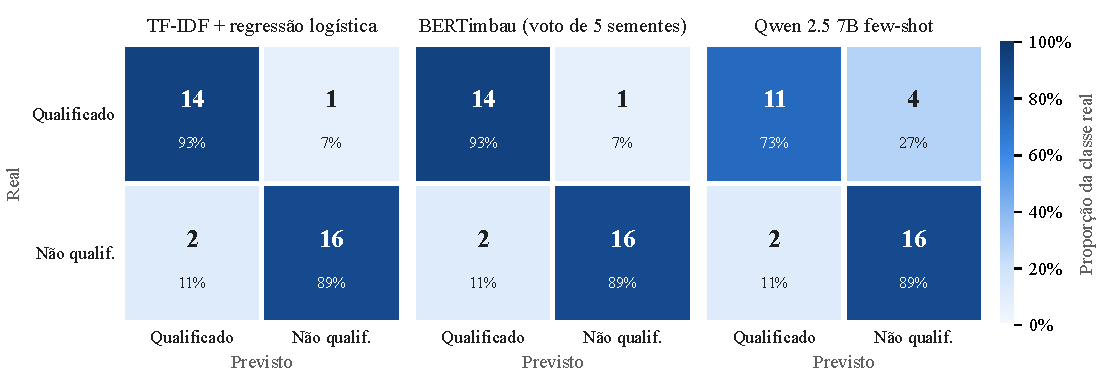
\includegraphics[width=\textwidth]{cm_qualificacao.pdf}
\fonte{Elaborado pelo autor (2026). Linhas: classe real; colunas: classe prevista. A cor e o percentual indicam a proporção da classe real. Para o BERTimbau, voto majoritário das cinco sementes.}
\end{figure}

\begin{figure}[htbp]
\centering
\caption{Matrizes de confusão da presença de objeção no conjunto de teste ($n = 33$)}
\label{fig-cm-objecao-presenca}
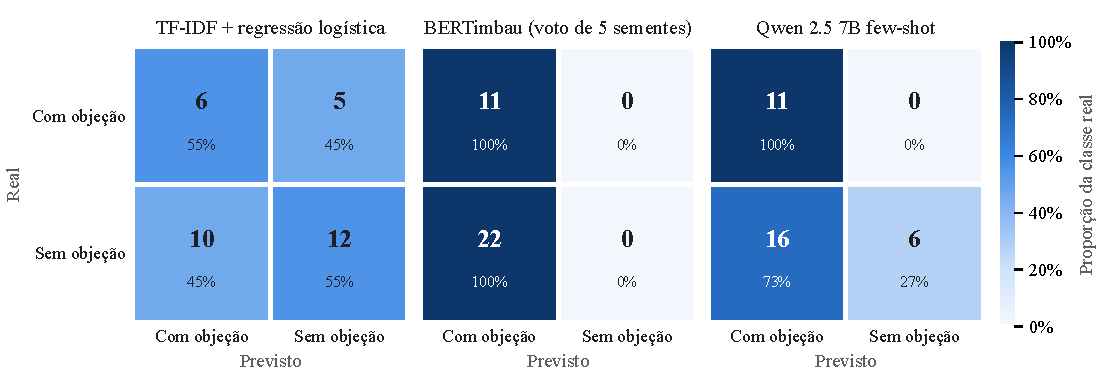
\includegraphics[width=\textwidth]{cm_objecao_presenca.pdf}
\fonte{Elaborado pelo autor (2026). Uma conversa é considerada com objeção quando ao menos uma categoria é atribuída.}
\end{figure}

\begin{figure}[htbp]
\centering
\caption{Matrizes de confusão por categoria de objeção no conjunto de teste ($n = 33$)}
\label{fig-cm-objecao-rotulos}
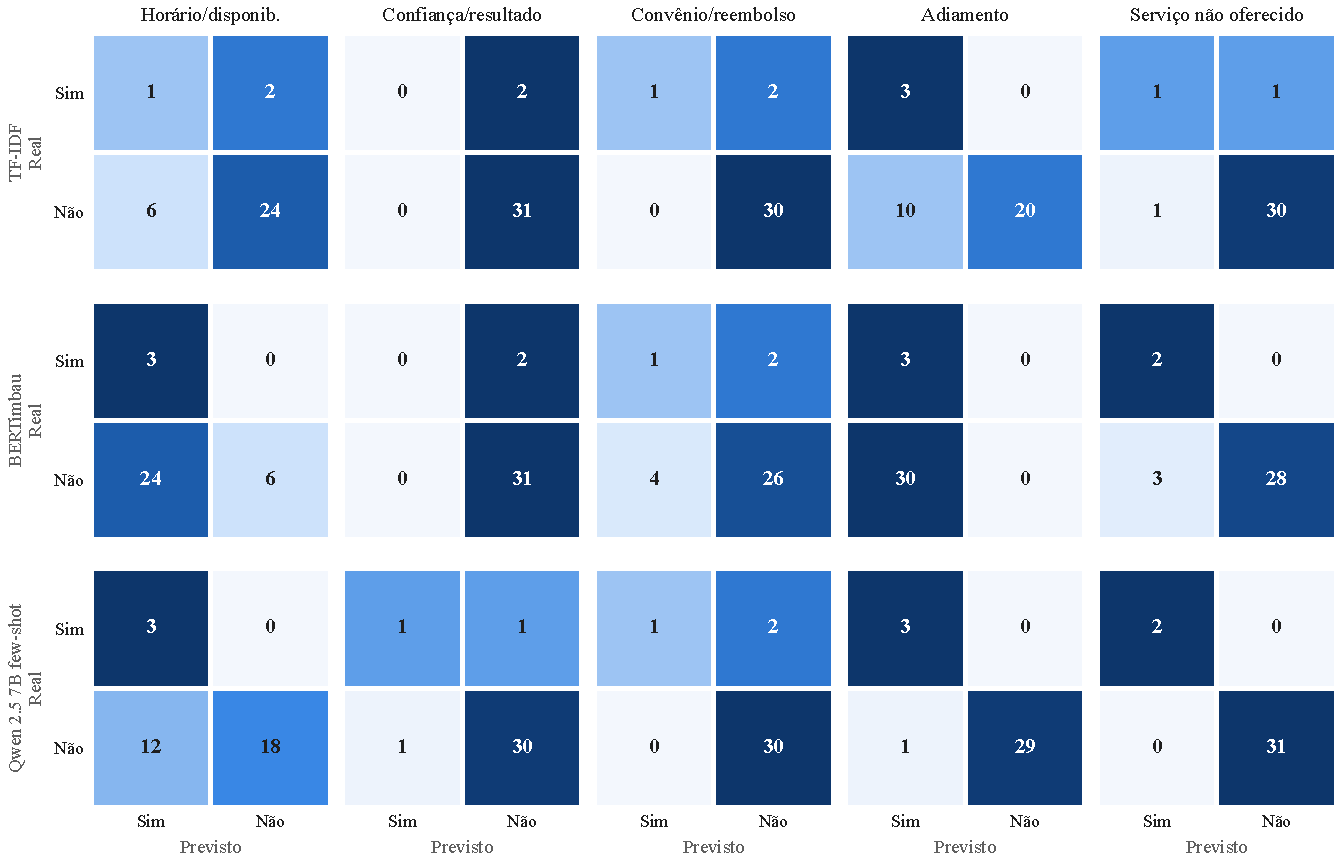
\includegraphics[width=\textwidth]{cm_objecao_rotulos.pdf}
\fonte{Elaborado pelo autor (2026). Apenas as categorias com ocorrência no teste. Linhas: categoria presente na referência; colunas: categoria prevista.}
\end{figure}
